\chapter{State of the art} \label{sec:colours}

Text-to-image is an emerging field of deep learning where models can generate lifelike and highly detailed images from textual descriptions.  The development of these models is a challenging task that requires the close integration of both computer vision and NLP approaches. The latest advancements in text-to-image models have led to the capability of producing high-quality images with rich semantic content that can now be used for tons of applications including video games and virtual reality, e-commerce, or education among others. Even though recent advancements have allowed the use for commercial applications, generative models remain a challenging and tough problem. This section aims to analyse the current state-of-the-art of text-to-image models

\section{Historical review of text-to-image models}

\section{Diffusion probabilistic models} \label{Dprobabilistic}

Throughout 2022, the capabilities and popularity of text-to-image models have exploded. The general public is aware of some models, such as DALL-E 2, Midjourney, or Stable Diffusion. Nonetheless, the vast majority of people are unaware of the technical prowess required in the field of Artificial Intelligence for these models to exist. This section aims to shed some light on the internal functioning and processes of these models from an academic perspective.

Diffusion probabilistic models are a class of latent variable models that introduce the ideas of nonequilibrium thermodynamics into data generation techniques by homogeneously adding noise into samples. Thus, they join the list of models that manage to generate high-quality images such as variational autoencoders (VAEs) or Generative adversarial networks (GANs). The latter models have been the reference of academic research in recent years and are the benchmark to be surpassed by diffusion models. 

GANs were introduced in 2014 by researchers at the University of Montreal in the paper \textit{Generative Adversarial Nets} \cite{goodfellow2020generative}. The idea is to create generative models through an adversarial process in which two neural networks compete against each other.  One of the networks will be generative while the other will be discriminative. Thus, the generative network will be in charge of capturing the distribution of the training dataset while the discriminative network must distinguish whether a sample comes from the generative network or the training data. The idea is that the generative network maximises the probability that the discriminative network makes errors. 

Diffusion models, on the other hand, achieve high-quality image synthesis results in the paper \textit{Denoising Diffusion Probabilistic Models} \cite{ho2020denoising} by researchers from the University of California, Berkeley. These models are based on creating a Markov chain in which at each step they add Gaussian noise to an image in a diffusion process and then learn to undo it. In this way, a network is trained that is capable of reconstructing images from random noise. The differences between GANs and diffusion models are presented in figure \ref{fig:GansvsDM}.

\begin{figure}
    \centering
    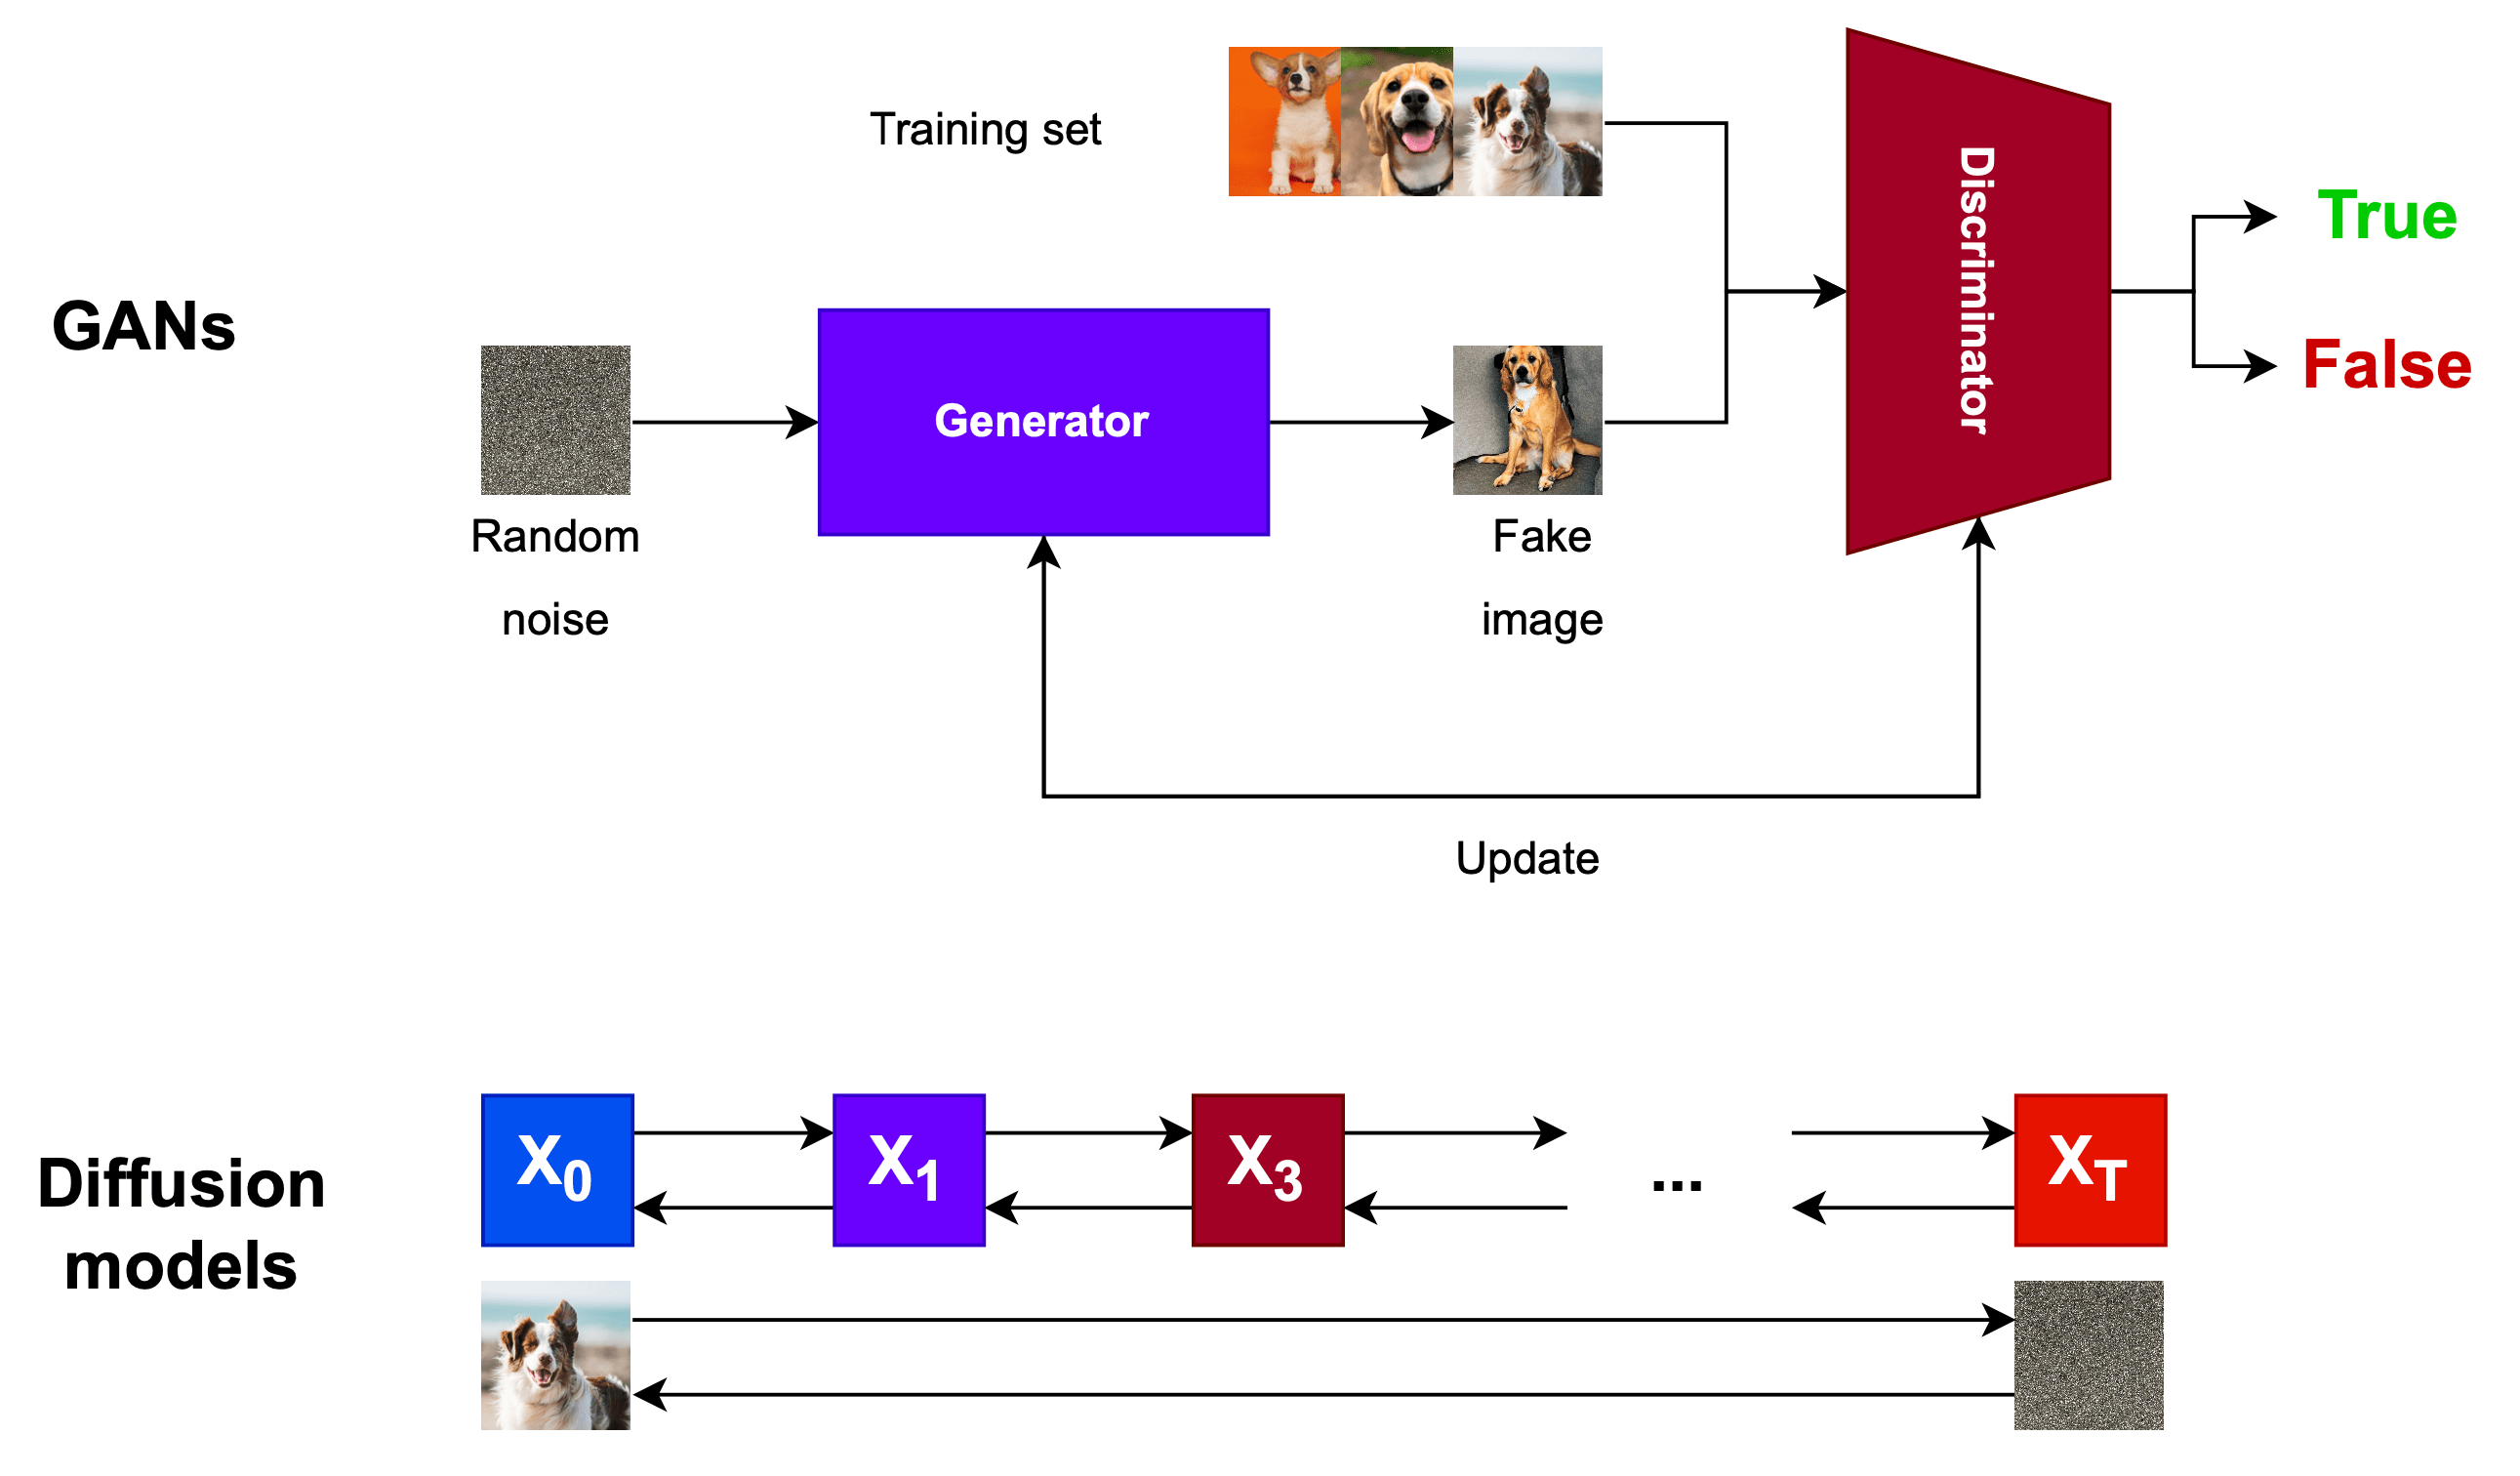
\includegraphics[width=0.75\textwidth]{Pictures/GansvsDM} 
    \caption{Overview of GANs and diffusion models}
    \label{fig:GansvsDM}
\end{figure}

Diving further into the workings of diffusion models, we define the \textbf{forward process} of the Markov chain. The first step is to take a sample of the target data distribution, which we will call $X_0$, and add Gaussian noise in $T$ steps. The forward process is thus defined as a Markov chain in which the state of a sample at time $n$ depends only on the state at time $n-1$. Therefore, one can denote the distribution of any sample conditioned on the initial state $X_0$.

\[ q\left(x_{1:T}\middle| x_0\right)=\prod_{t=1}^{T}{q\left(x_t\middle| x_{t-1}\right)} \]

In every step of the noising process Gaussian noise is added according to some variance schedule $\beta_1...\beta_t$, normally consider as hyperparameters. The restrictions applied to $\beta_t$ are $\beta_1 < \beta_2 ... < \beta_t$ and $\beta_t \epsilon (0, 1)$. $I$ stands for identity.

\[q\left(x_t\middle| x_{t-1}\right)=\mathcal{N}\left(x_t;\sqrt{1-\beta_tx_{t-1}},\beta_tI\right) \]

As $\beta_t$ grows in time and $T$ approaches the limit ($T \rightarrow\infty$, $\beta_t \rightarrow 0$), the Gaussian mean will approach zero with identity covariance. In this way, the distribution will lose all the information contained in the original image. In practice, researchers use a $T$ close to 1000 \cite{ho2020denoising}.

\[q\left(x_t\middle| x_0\right)\approx\mathcal{N}\left(0,I\right)\]

Figure \ref{fig:MarkovchainDP} shows the diffusion process described so far.

\begin{figure}
    \centering
    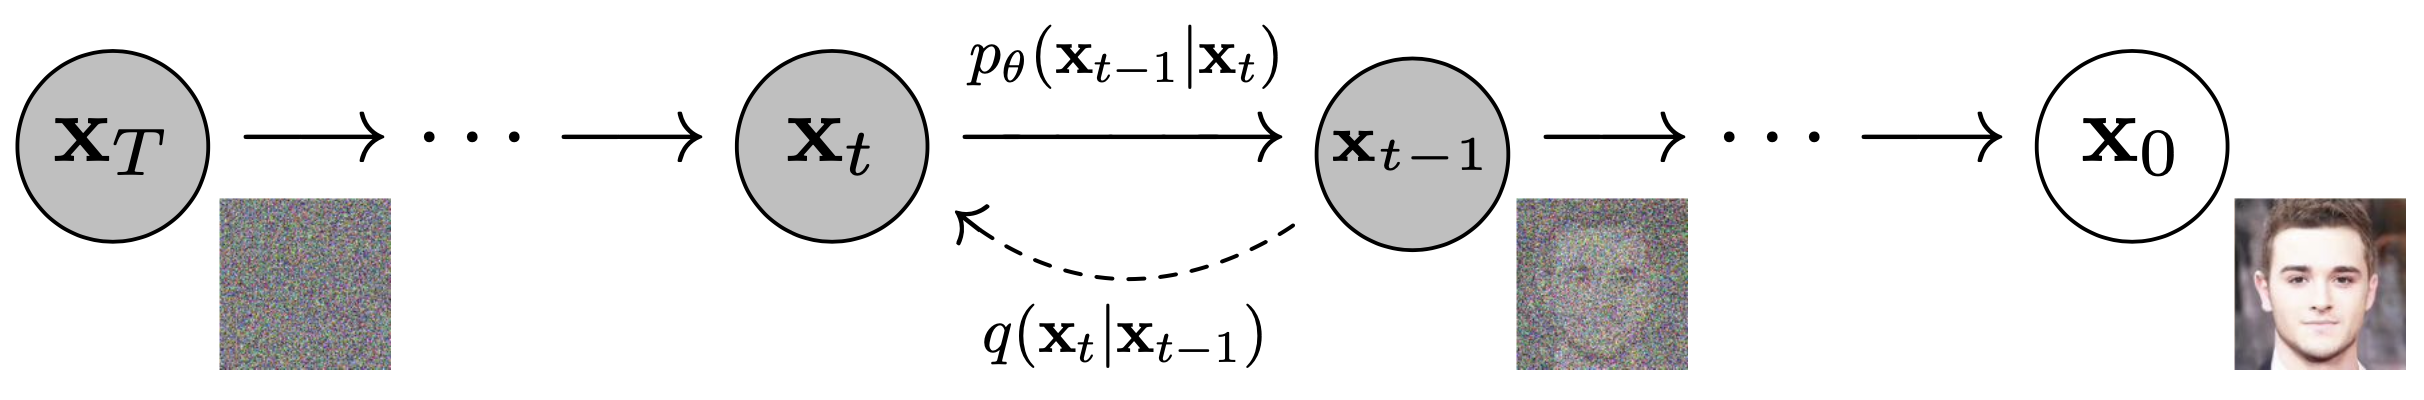
\includegraphics[width=0.75\textwidth]{Pictures/MarkovchainDP} 
    \caption{Markov chain of the diffusion process \cite{ho2020denoising}}
    \label{fig:MarkovchainDP}
\end{figure}

In summary, it is proven that the forward process destroys the structure of a data distribution step by step. The next challenge is to learn the \textbf{reverse diffusion process} in order to generate data that resembles the training distribution from pure Gaussian noise. As with the forward process, the reverse diffusion process can be expressed as a Markov chain where the probability of a sequence of samples can be expressed as the product of conditional probabilities.

\[ p_\theta\left(x_{0:T}\right) := p\left ( x_T \right ) \prod_{t=1}^{T}p_\theta\left ( x_{t-1} | x_t\right ) \]

The reverse diffusion process involves a neural network to remove noise from an image in a stepwise manner. Thus, starting from pure Gaussian noise, noise is removed step by step to arrive at an image that resembles the training distribution. The reason that the process has to be done in a stepwise manner is that "\textit{the estimation is more tractable than explicitly describing the full distribution}" as expressed in the publication \textit{Deep Unsupervised Learning using Nonequilibrium Thermodynamics} \cite{sohl2015deep}.

The neural network that the authors of DDPM propose aims to \textbf{predict the noise to subsequently eliminate it from the image}. This is equivalent to obtaining the mean of the distribution since the authors decide to fix the variance. The authors decide to use the \textbf{U-Net network} \cite{ronneberger2015u} for this purpose. U-Net consists of a bottleneck in the middle that ensures that the network removes irrelevant information and focuses on the important information. In addition, the network, between the encoder and the decoder, uses residual connections to improve efficiency. Finally, the authors of DDPM decide to employ self-attention at the 16 × 16 feature map resolution. Figure \ref{fig:ReverseDP} shows a schema of the learning process.

\begin{figure}
    \centering
    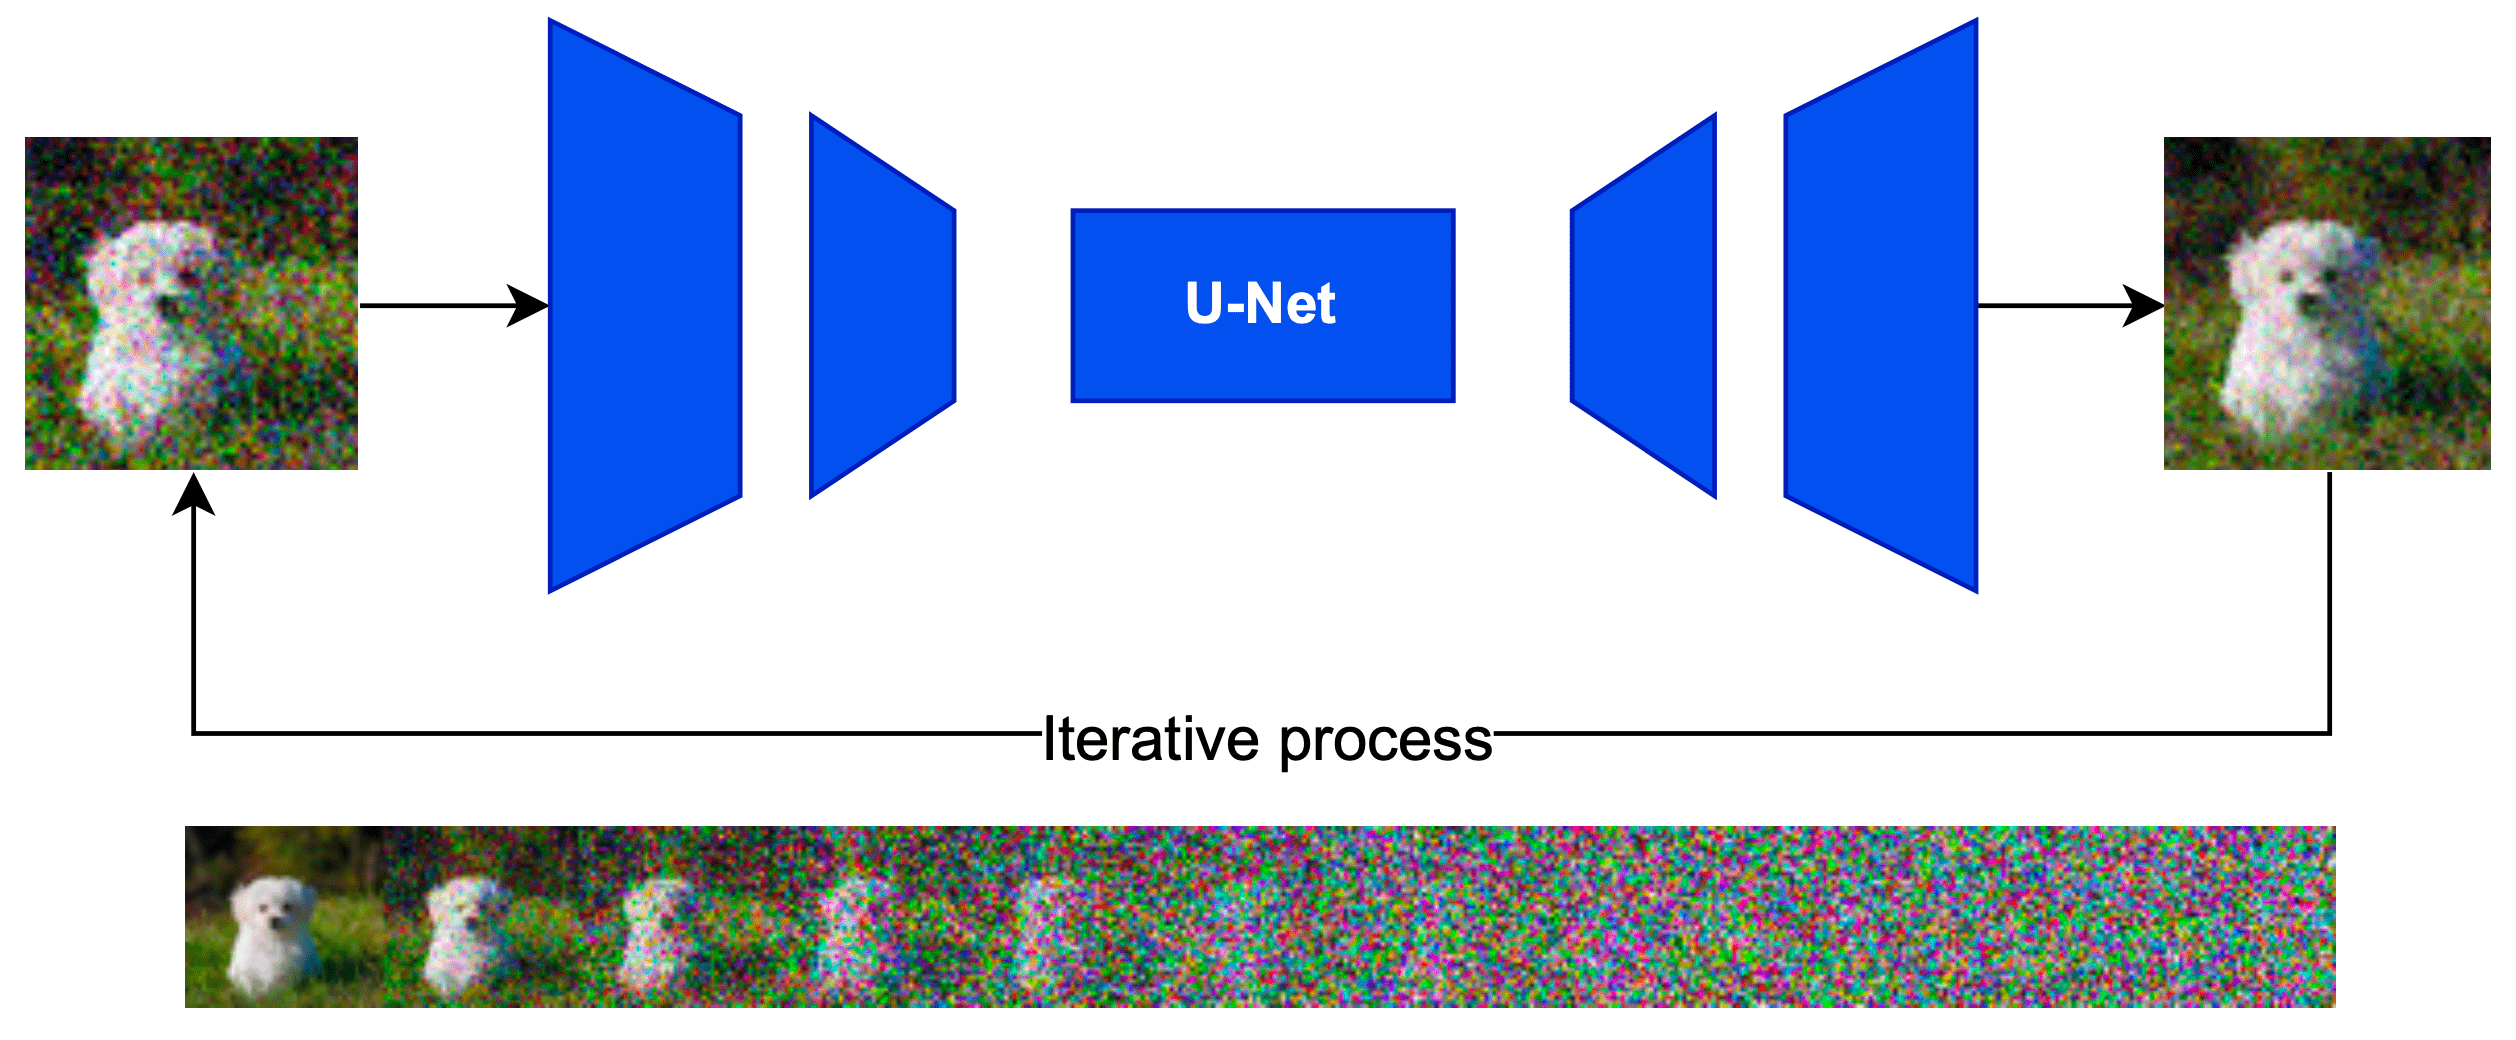
\includegraphics[width=0.75\textwidth]{Pictures/ReverseDP.png} 
    \caption{Reverse diffusion learning schema}
    \label{fig:ReverseDP}
\end{figure}

Another question that arises when working with diffusion models is how conditional generations can be provided. This can be achieved through various techniques. One way is to feed a conditional variable into the training so that the model makes use of it in the generation to resemble a subset of the training distribution. However, guiding the generation process through a classifier is a more flexible technique that allows even more complex text descriptions than simple labels to be worked with. The idea is to take an already trained classifier and \textbf{guide the generation in the direction of the gradient of the classifier label}.

\subsection{Improvements to diffusion probabilistic models }

Although the results obtained by the \textit{Denoising Diffusion Probabilistic Models} \cite{ho2020denoising} paper are excellent and represent a great leap forward compared to the images that the generative models were capable of generating until then, researchers at OpenAI suggest some improvements that increase the quality of the results in their publication \textit{Improved Denoising Diffusion Probabilistic Models} \cite{nichol2021improved}. In it, the main improvements they propose to the model are \textbf{(i) the incorporation of learned variances and (ii) an improvement of the noise schedule}. 

As discussed in section \ref{Dprobabilistic}, the authors of the paper \textit{Denoising Diffusion Probabilistic Models} \cite{ho2020denoising} decided to fix the variance. However, the OpenAI researchers decide to learn the interpolation of the variance between an upper and lower bound. This allows them to maintain the quality of the samples and improve the log-likelihood. Finally, they modify the loss to depend on the variance by a scaling factor $\lambda$ set experimentally to 0.001.

On the other hand, the OpenAI authors present a new noise schedule designed to be linear in the central region and have little change at the beginning and end. It is defined through $ \bar{\alpha_t}$, affecting the definition of the variances $\beta_t$ as follows.

\[\beta_t = 1 - \frac{\bar{\alpha}_t}{\bar{\alpha}_{t-1}}\]

The proposed cosine noise schedule can be seen in figure \ref{fig:CosineSC}. Whereas, figure \ref{fig:CosineEX} shows how each of the schedules adds noise to the image. The \textbf{linear schedule destroys the information faster and presents a sub-optimal behaviour} since the last steps are practically pure noise. Thus, the cosine schedule is superior as it allows a more controlled addition of noise.

\begin{figure}
    \centering
    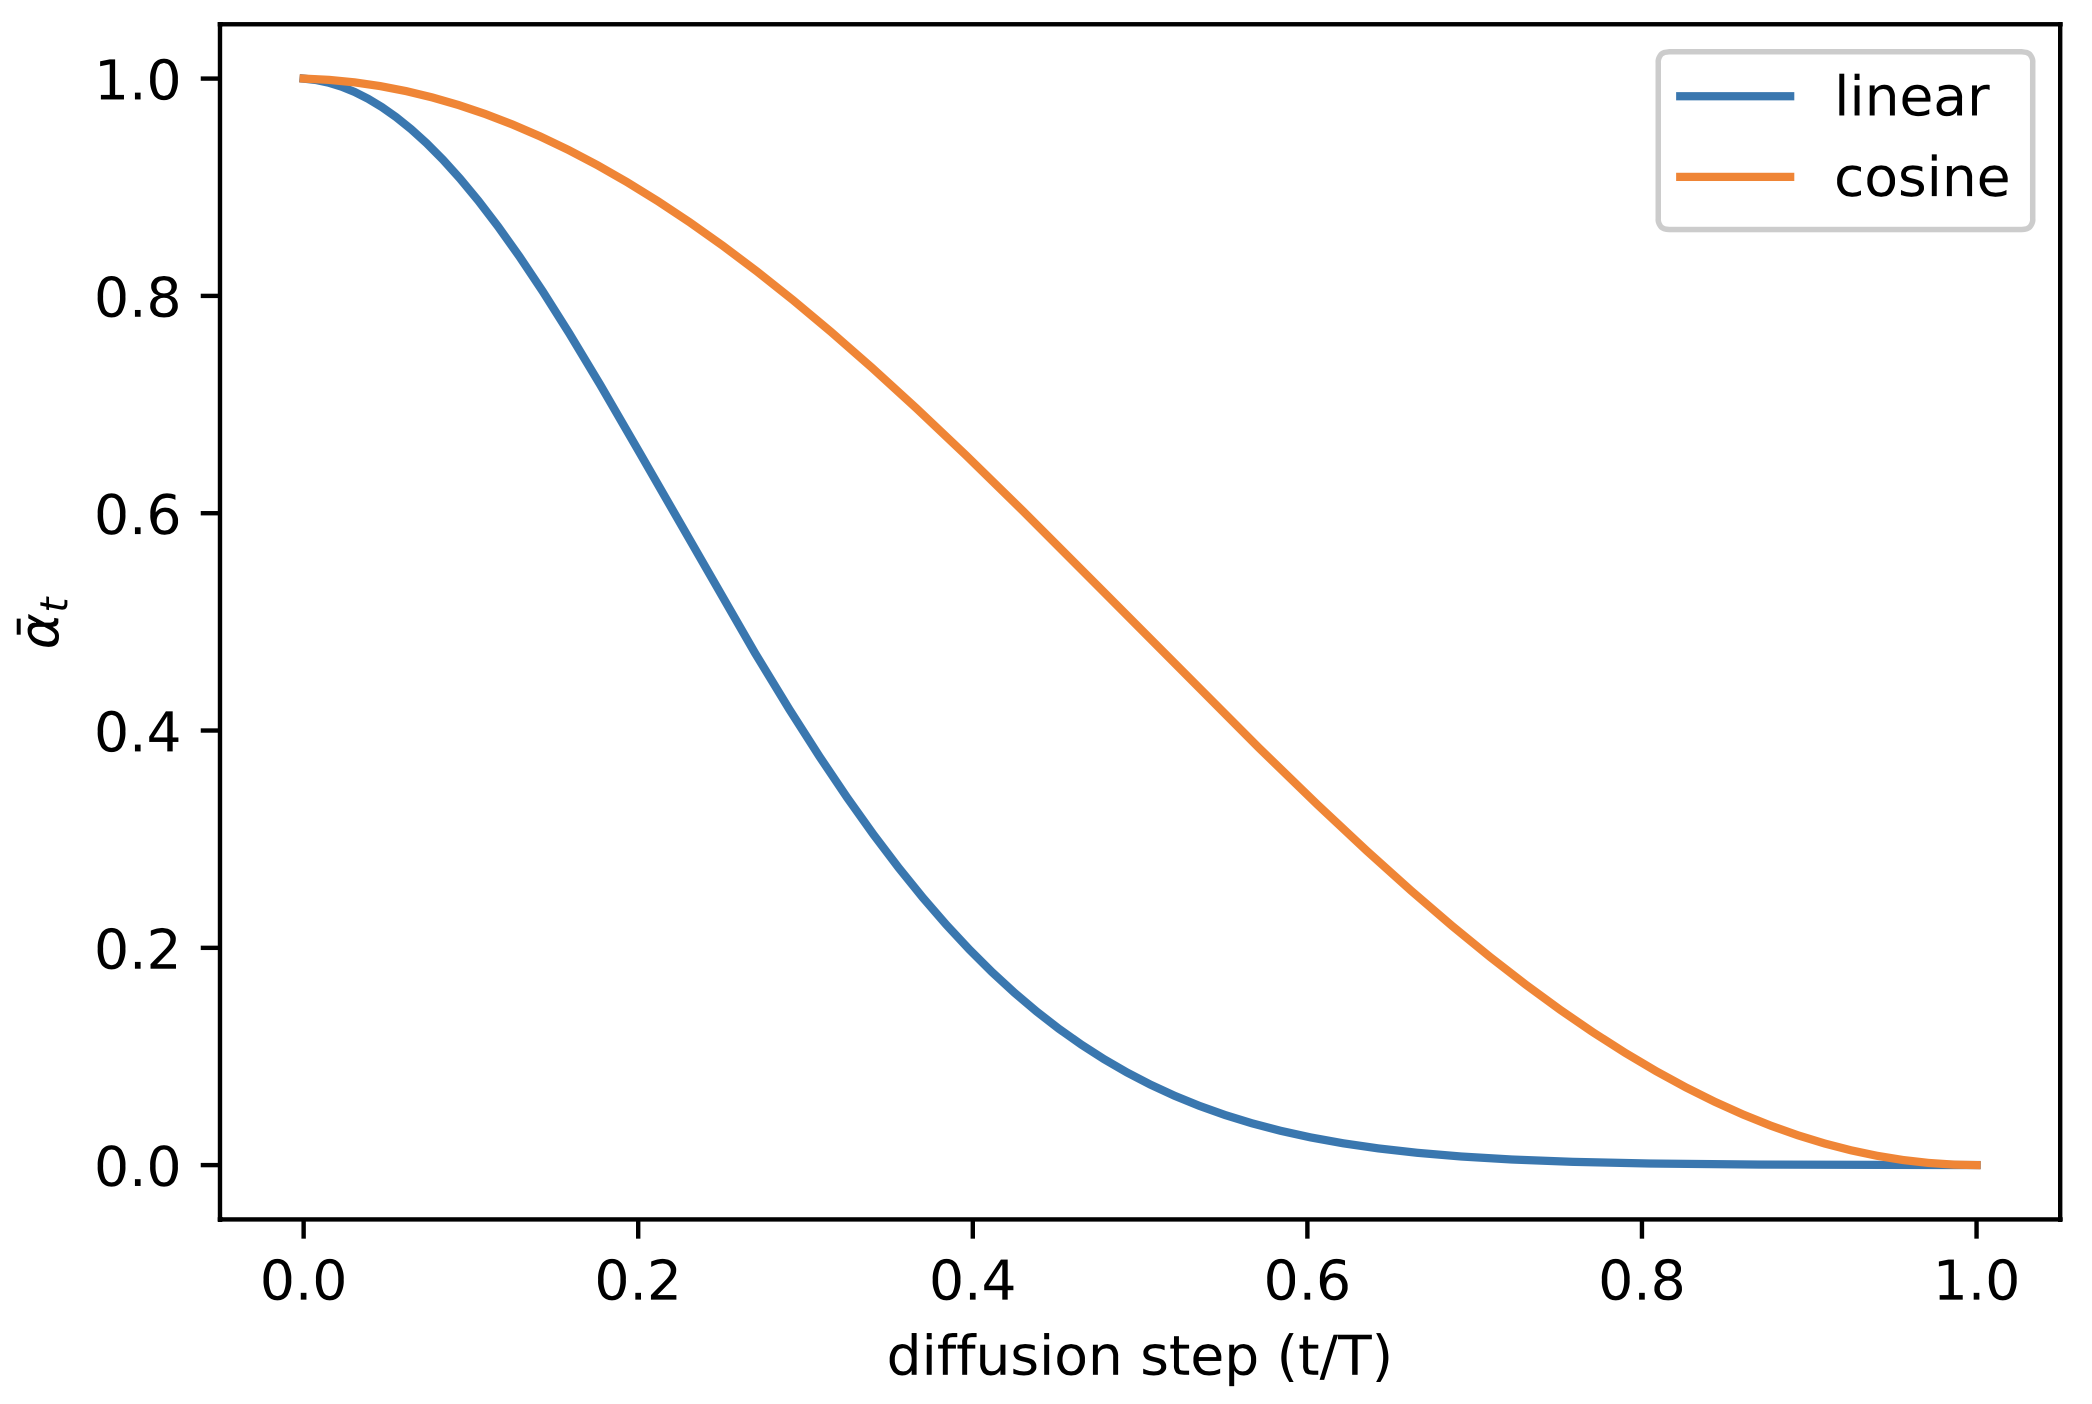
\includegraphics[width=0.5\textwidth]{Pictures/cosineSC.png} 
    \caption{Cosine and linear schedules comparison}
    \label{fig:CosineSC}
\end{figure}

\begin{figure}
    \centering
    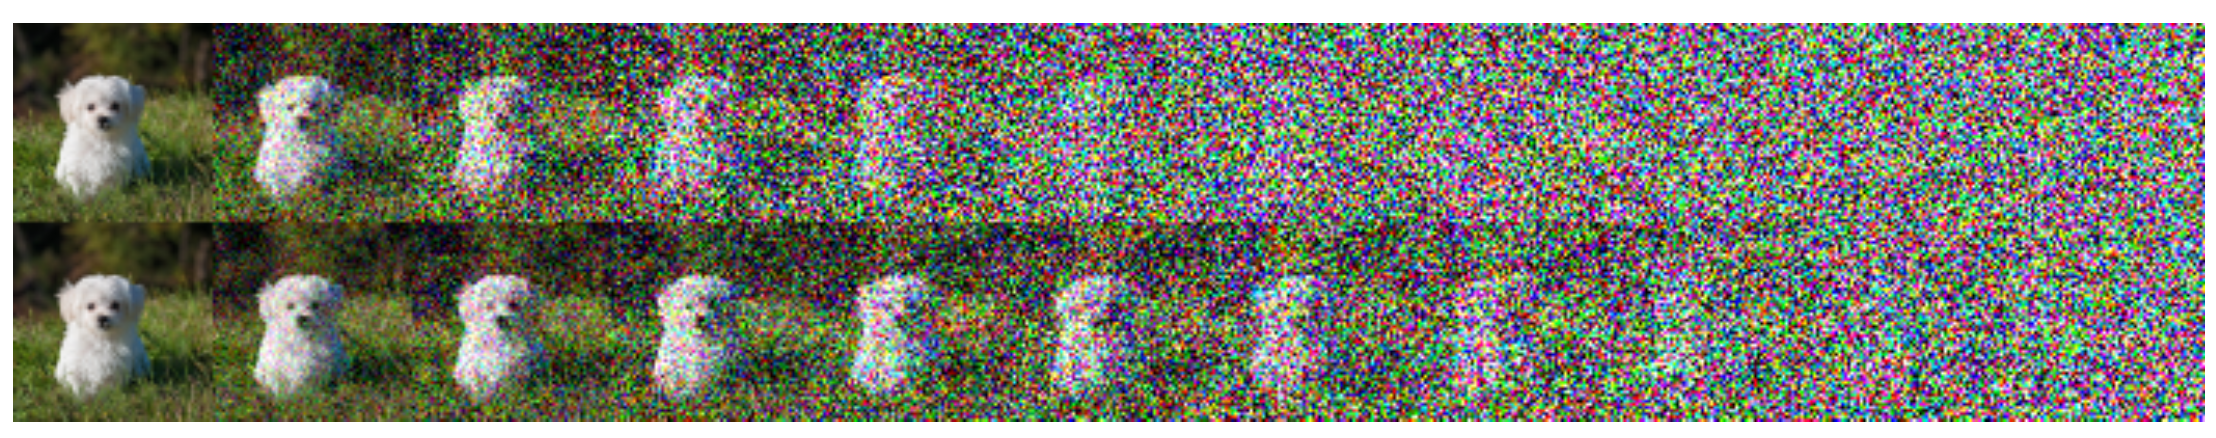
\includegraphics[width=0.75\textwidth]{Pictures/cosineEX.png} 
    \caption{Cosine (bottom) and linear (top) schedules comparison on an image}
    \label{fig:CosineEX}
\end{figure}

However, the improvements do not stop there. The same OpenAI researchers in a later paper called \textit{Diffusion Models Beat GANs on Image Synthesis} \cite{dhariwal2021diffusion} demonstrate how a series of modifications to the architecture and the use of classifier guidance can produce images that are better than the state of the art at the time. The enhancement they make to the architecture are:

\begin{itemize}
    \item \textbf{Increasing the depth while decreasing the width} to keep the size of the model relatively constant.
    \item Increased use of \textbf{attention heads and layers}
    \item Upsampling and downsampling the activations by means of the \textbf{BigGAN residual blocks} \cite{brock2018large}.
    \item Use of \textbf{adaptive group normalization} (AdaGN) layers, in which the concept of group normalization is expanded by adjusting the normalization parameters of each group separately according to the input data.
    \item \textbf{Classifier guidance}. Employing an additional classifier, the diffusion model is assisted in generating a certain class.
\end{itemize}

\section{Latent diffusion models}

\section{Stable diffusion} \label{SD}

\subsection{Training dataset}

A significant challenge posed by models like Stable Diffusion is the choice of images they are trained on. This issue is not insignificant as image generation models require both textual descriptions of training images and a sufficient amount of variety to enable the model to comprehend how the world is constructed and thus be capable of reproducing it. However, the conventional datasets of the Machine Learning field (COCO, ImageNet, etc) fail to satisfy these requirements since they are not intended for this purpose. Researchers have discovered that the solution is the web, where a vast array of diverse images about the world can be found, many of which have HTML alt attribute tags.

Stable Diffusion has an advantage over some of its rivals, including \textit{DALL-E 2}, in that it is an open-source project, meaning that the dataset employed for training is well-known and accessible to everyone. Specifically, the dataset used by Stable Diffusion is "\textit{\textbf{LAION-5B}, a dataset of 5.85 billion CLIP-filtered image-text pairs, 14x larger than \textbf{LAION-400M}, previously the biggest openly accessible image-text dataset in the world}" \cite{schuhmann2022laion}. In particular, Stable Diffusion presents several checkpoints on various LAION-5B assemblies. Some of these checkpoints in Stable Diffusion version 1 \cite{SDCardHF} are:

\begin{itemize}
  \item \textbf{stable-diffusion-v1-1}: 256 x 256 images from a subset of 2.3 billion English-captioned images called \textbf{LAION-2B-EN}.
  \item \textbf{stable-diffusion-v1-2}: Resumed training on \textit{stable-diffusion-v1-1} with 512x512 images from the subset \textbf{LAION-2B-EN}, containing a selection of improved aesthetics images compared to the others.
  \item \textbf{stable-diffusion-v1-3}: Resumed training on \textit{stable-diffusion-v1-2} with the same subset of images but a 10\% dropping of the text-conditioning.
  \item \textbf{stable-diffusion-v1-4}: Resumed training on \textit{stable-diffusion-v1-2} with 512x512 images from the subset \textbf{LAION-Aesthetics v2 5+}, containing 600 million images from \textbf{LAION-2B-EN} with better aesthetics and low-resolution and watermarked images filtered out.
  \item \textbf{stable-diffusion-v1-5}: \textit{stable-diffusion-v1-4} trained with more steps.
\end{itemize}

LAION-5B retrieves images from the internet that are not uniformly high in quality. Because these images are gathered automatically, they do not adhere to the same rigorous standards as other image datasets. As a result, the checkpoints for training Stable Diffusion use varying subsets of LAION-5B. Nonetheless, the fact that the images obtained are not accurately labelled as they are in standard vision supervised learning is actually an advantage. Consequently, Stable Diffusion is now included in the group of architectures, such as CLIP or DALL-E 2, that have proven the value of these vast datasets, even though they contain a significant amount of noise.

LAION-5B contains 5.85 billion image-text pairs divided into three subsets. \textbf{LAION2B-EN}, which contains 2.32 billion English image-text pairs; \textbf{LAION2B-MULTI} with 2.26 billion image-text pairs from all other languages (Russian, French and German as top 3) and \textbf{LAION1B-NOLANG} of 1.27 billion samples where the language is not correctly defined. 

\subsubsection{LAION-5B Description}

The attributes that can be found in LAION-5B are described in table \ref{table:TableLaionAttributes}.

% Please add the following required packages to your document preamble:
% \usepackage[table,xcdraw]{xcolor}
% If you use beamer only pass "xcolor=table" option, i.e. \documentclass[xcolor=table]{beamer}
\begin{table}[ht]
\centering
\begin{tabular}{|p{0.25\linewidth} | p{0.65\linewidth}|}
\hline
{\textbf{Attribute}} & {\textbf{Description}} \\ \hline
\textbf{id} & Image identifier \\ \hline
\textbf{URL} & URL from where the image was obtained \\ \hline
\textbf{Text string} & Caption accompanying the image \\ \hline
\textbf{Dimensions} & Height and width of the image \\ \hline
\textbf{Similarity} & Cosine similarity between the text and image embeddings. CLIP-based   models are employed to gauge the level of accuracy with which an image is   described by a given textual description.\\ \hline
\textbf{pwatermark} & Probability that the image presents a watermark. The value is   obtained by a custom model trained by LAION. Value between 0 and 1 \\ \hline
\textbf{punsafe} & Probability that the image is NSFW. As some of the content   acquired from the web may not be suitable for all audiences, LAION employs a   custom model to assess its adequateness. Value between 0 and 1 \\ \hline
\end{tabular}
\caption{LAION-5B’s attributes}
\label{table:TableLaionAttributes}
\end{table}

Some statistics of the subsets computed by the LAION team can be found in table \ref{table:TableLaionStatistics} \cite{schuhmann2022laion}.

\begin{table}[ht]
\begin{tabular}{|l|l|l|l|l|}
\hline
\textbf{Subset} & \textbf{Dimensions} & \textbf{NSFW} & \textbf{Watermark} & \textbf{Average text length} \\ \hline
\textit{LAION2B-EN} & \begin{tabular}[c]{@{}l@{}}-   \textgreater{}256x256: 1324M\\    \\ -   \textgreater{}512x512: 488M\\    \\ -   \textgreater{}1024x1024: 76M\end{tabular} & 2.9\% & 6.1\% & 67 \\ \hline
\textit{LAION2B-MULTI} & \begin{tabular}[c]{@{}l@{}}-   \textgreater{}256x256: 1299M\\    \\ -   \textgreater{}512x512: 480M\\    \\ -   \textgreater{}1024x1024: 57M\end{tabular} & 3.3\% & 5.6\% & 52 \\ \hline
\textit{LAION1B-NOLANG} & \begin{tabular}[c]{@{}l@{}}- \textgreater{}256x256:   1324M\\    \\ -   \textgreater{}512x512: 488M\\    \\ -   \textgreater{}1024x1024: 76M\end{tabular} & 3\% & 4\% & 46 \\ \hline
\end{tabular}
\caption{Statistics summary for LAION-5B}
\label{table:TableLaionStatistics}
\end{table}

By analysing the data presented in tables \ref{table:TableLaionAttributes} and \ref{table:TableLaionStatistics}, one can infer the rationale behind the various checkpoints employed in the Stable Diffusion model. The LAION-5B dataset, owing to its extensive diversity, can be partitioned into subsets that cater to various generation objectives. As a result, the model can be adapted to different resolutions or the quality of the generated images can be adjusted by filtering out low similarity image-to-description pairs, NSFW content, or watermarked content.

It is noteworthy to mention that the primary characteristics of the entries in the dataset are produced by other pre-trained models. This highlights the significance of incorporating other models in the data collection process for large AI models, as they can assist in adding supplementary features to the dataset. A more detailed discussion of this fact can be found in section \ref{LCollection}

\subsubsection{LAION-5B Collection Methodology} \label{LCollection}

The pipeline followed when creating the LAION-5B dataset involves: (i) obtaining Common Crawl data, (ii) filtering some web pages, (iii) downloading the image-text pairs, (iv) and filtering the content according to various characteristics.

Common Crawl is an organization dedicated to web crawling, data collection, and storage. It makes all the gathered data publicly available. In the October 2022 crawl, the total file size was 380 TBs, comprising 3.15 billion web pages. The dataset's key feature is that it contains HTML tag information about the images, including the "alt" attribute, which provides an alternative description of the images. This attribute is widely used on the web, for example, to address page rendering issues, assist visually impaired individuals, or aid web content indexing by search engines. Therefore, it is a ubiquitous attribute on the web that is encouraged to improve page usability and ranking in web search engines.

After the Common Crawl data is accessible, images that have information in the "alt" attribute are chosen. Once both images and descriptions are available, a language detection model is employed on the descriptions, and the data is then divided into three subsets: LAION2B-EN, LAION2B-MULTI, and LAION1B-NOLANG, as mentioned earlier. It is noteworthy that in order to incorporate data into LAION1B-NOLANG, a confidence threshold is determined based on the prediction of the language detection model, and if it is insufficient, it is included in this subset.

The next step is to clean the dataset of poor-quality images and descriptions. For this purpose, images, and descriptions with less than 5KB data, 5 words and 0.28 cosine similarity (in LAION2B-EN) are removed. \textbf{The cosine similarity is computed thanks to Open AI's CLIP model, which computes the embedding of images and text.}

It is important to notice the importance of the CLIP contrastive model in understanding how the Stable Diffusion training dataset was created. As explained above, CLIP is able to associate images and text. The way in which it achieves this is very clever as it can solve the classic problem of labels in Deep Learning. Thus, CLIP is a pioneer in bringing together language models and vision models by making supervision in natural language. And therein lies the key to LAION-5B: unlike other datasets that require a specialized team to create carefully curated tags, this dataset relies on natural language descriptions provided by internet users. This allows for much faster scalability. It is worth noting that CLIP is not only essential in the creation of the dataset, but it also plays a vital role in the Stable Diffusion model, as previously explained in section \ref{SD}.

The final stage of the pipeline involves incorporating additional attributes that help categorize the image in a useful way, beyond just its similarity to text. One such attribute is the probability that the image contains NSFW content, which is determined using a custom model. Another attribute is the probability that the image has a watermark, which is determined using a separate model designed for that purpose.

Summing up, the creation of LAION-5B relies on multiple AI models that help gather reliable content from the internet and guarantee the accuracy of image descriptions. This marks a significant shift in the way we collect data for training models, where the emphasis is on scaling the dataset rather than carefully generating accurate labels. Instead, models like CLIP enable the use of natural language descriptions that accompany web images for data collection.

\section{Subject-driven generation techniques}

